\documentclass[10pt]{article}

\usepackage{answers}
\usepackage{setspace}
\usepackage{graphicx}
\usepackage{enumitem}
\usepackage{multicol}
\usepackage{circuitikz}
\usepackage{adjustbox}
\usepackage{mathrsfs}
\usepackage{mathtools}
\usepackage{fancyhdr}
\usepackage{svg}
\usepackage[margin=1in]{geometry}
\usepackage{amsmath,amsthm,amssymb}
\usepackage[compact]{titlesec}
\titlespacing{\section}{0pt}{*0}{-10pt}
\titlespacing{\subsection}{0pt}{*0}{-10pt}
\titlespacing{\subsubsection}{0pt}{0pt}{-10pt}
\parindent 0in
\parskip 12pt
\setlength{\headsep}{-10pt}
\setlength{\topskip}{0pt}
\setlength{\topmargin}{0pt}
\setlength{\topsep}{0pt}
\setlength{\partopsep}{0pt}
\geometry{margin=1in, headsep=0.25in}
\setlist[itemize]{label={--}, topsep=-10pt, noitemsep}
\setlist[enumerate]{topsep=-10pt, noitemsep}
\newcommand{\N}{\mathbb{N}}
\newcommand{\Z}{\mathbb{Z}}
\newcommand{\C}{\mathbb{C}}
\newcommand{\R}{\mathbb{R}}


\pagestyle{fancy}
\lhead{Aditya Arora}
\rhead{page \thepage}
\cfoot{ECE 222 Digital Computers}
\renewcommand{\headrulewidth}{0.2pt}
\begin{document}
\section*{Memory System}
The size of a memory is determined by the number of unique addressable memory locations.
$$k \text{ address bits} = 2^k \text{ addresses}$$
\textbf{Memory Access Time:} the time that elapses between the initiation of an operation to transfer a word of data and the completion of that operation. This is referred to as the memory access time\\
\textbf{Memory Cycle Time:} the minimum time delay required between the initiation of two successive memory operations\\
\textbf{RAM:} A memory unit is called a random-access memory (RAM) if the access time to any location is the same, independent of the location’s address. \\
\textbf{Cache memory:}  a small, fast memory inserted between the larger, slower main memory and the processor. It holds the currently active portions of a program and their data.\\
\textbf{Virtual memory:} With this technique, only the active portions of a program are stored in the main memory, and the remainder is stored on the much larger secondary storage device. Sections of the program are transferred back and forth between the main memory and the secondary storage device in a manner that is transparent to the application program.\\
\textbf{Block Transfers:} transfers between the main memory and the cache and between the main memory and the disk do not occur one word at a time. Data are always transferred in contiguous blocks involving tens, hundreds, or thousands of words.
$$\text{bandwidth} = \text{words} \times \frac{\text{bytes}}{word} \times \frac{\text{frequency}}{\text{cycles}}$$
Number of cycles:
\begin{enumerate}
    \item Async DRAM: $= (RAS + CAS + 1) \times burst\; size$
    \item Fast page mode DRAM $= \Big((RAS + CAS + 1)\times 1 + (CAS + 1) \times (burst\; size -1)\Big)$
    \item Synchronous DRAM (SDRAM) $= {RAS + CAS + burst\; size}$
    \item DDR - SDRAM: $=RAS + CAS + \frac{burst\; size}{2}$
\end{enumerate}
\textbf{Memory Sizes}:
\begin{itemize}
    \item KiB: $2^{10} = 1024\; bytes$
    \item MiB: $KiB^2 = 1024^2\; bytes$
    \item GiB: $KiB^3 = 1024^3\; bytes$
    \item TiB: $KiB^4 = 1024^4\; bytes$
\end{itemize}
offset bits = $log_2(Block\; Size)$\\
The first and the last address can be generated by having offsets 000000, 111111 be concatenated with the block address.\\
Direct-mapped cache:
\begin{itemize}
    \item offset bits: $log_2$(block size)
    \item index: $log_2$(number of blocks)
    \item Tag: number of address bits - (index bits + offset bits)
\end{itemize}
number of cache lines = $\frac{Cache\;size}{Block\;size}$\\
N-way set-associative cache:
\begin{itemize}
    \item offset bits = $log_2$(block size)
    \item number of sets = number of cache lines / N
    \item index bits = $log_2$(number of sets)
    \item Tag = number of address bits - (index bits + offset bits)
\end{itemize}
\newpage
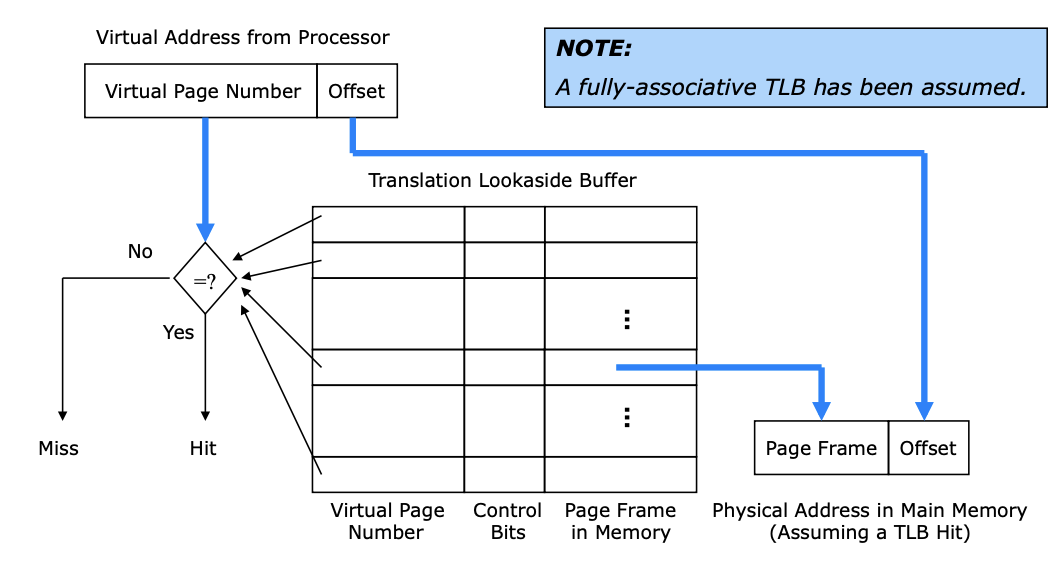
\includegraphics[width=0.8\textwidth]{memory/tlb.png}\\
Translation divides address bits into 2 fields
\begin{itemize}
    \item Lower bits give offset of word within page (page offset)
    \item Upper bits give virtual page number (vpn)
\end{itemize}
Page offset = $log_2$(page size)\\
\# of virtual page number (VPN) bits = \#virtual address bits - page offset\\
\# of physical page number (PPN) bits = \#physical address bits - page offset\\
It is possible to improve the performance of virtual memory
address translation by moving the page table into the MMU:
\begin{itemize}
    \item The entire page table is often too large to be stored within the MMU
    \item A portion of the page table, known as a translation lookaside buffer (TLB) is typically stored in the MMU and holds recently accessed entries of page table
    \item The TLB is analogous to a cache for page table entries
\end{itemize}
\end{document}
